\documentclass[11pt]{article}

% Handle Spanish seamlessly!
\usepackage[utf8]{inputenc}
\usepackage[spanish, es-tabla]{babel}

% Change the language for the captions and default names
\renewcommand{\figurename}{Figura}

% Needed for the multline environment
\usepackage{amsmath}

% Images
\usepackage{graphicx}
\graphicspath{{Img/}}

\usepackage{geometry}
\geometry{
    a4paper,
    left = 20mm,
    right = 20mm,
    top = 15mm,
    bottom = 15mm
}

% Links please!
\usepackage{hyperref}

% Format the links
\hypersetup{
    pdfborder = {0 0 0},    % Remove the ugly border
    colorlinks = true,      % Let there be color
    citecolor = black,      % Make citations appear normal (i.e black)
    linkcolor = black,      % The same for links (i.e table of contents)
    urlcolor = cyan         % Color the web links. (cyan is fancy for blueish...)
}

\title{Conformando trafico}
\author{Pablo Collado Soto \\ \\ \textit{Ingeniería de Tráfico}}
\date{}

\begin{document}
    \maketitle

    \section{Introducción}
        En esta práctica comenzaremos por estudiar el funcionamiento de un clasificador \textit{WFQ} de manera práctica a través de la simulación de un escenario análogo al de la práctica anterior. Más tarde analizaremos un clasificador \textit{WFQ} de manera teórica para terminar con el estudio de un conformador de tráfico según un cubo con goteo así como una función policía basada en el mismo algoritmo.

    \section{Estudiando un clasificador \textit{WFQ} (2.1.1)}
        Antes de nada definiremos los flujos de nuestro escenario en la tabla \ref{tab:wfqFlows}. Debemos tener en cuenta que la velocidad de la interfaz de salida de los flujos de datos es $V_l = 10\ Mbps$ para toda la prueba. La configuración del router para este escenario se puede encontrar \href{https://github.com/UAH-s-Telematics-Engineering-Tasks/traff_eng/blob/master/P2/Router_confs/originalWFQ.cfg}{aquí}.

        \begin{table}
            \centering
            \begin{tabular}{|c|c|c|c|c|c|c|}
                \hline
                & \texttt{Puerto} & \texttt{Comienzo [s]} & \texttt{Fin [s]} & \texttt{Tasa [Mbps]} & \texttt{Paquetes por segundo} & \texttt{SDU de UDP [B]}\\
                \hline
                1 & 51151 & 0 & 20 & 8 & 800 & 1250\\
                \hline
                2 & 51152 & 5 & 20 & 1,5 & 150 & 1250\\
                \hline
                3 & 51153 & 10 & 20 & 4 & 400 & 1250\\
                \hline
                4 & 51154 & 15 & 20 & 2,4 & 240 & 1250\\
                \hline
                5 & 51155 & 15 & 20 & 1,6 & 160 & 1250\\
                \hline
            \end{tabular}
            \caption{Configuración de los flujos para estudiar \textit{WFQ}.}
            \label{tab:wfqFlows}
        \end{table}

        \subsection{Comentando las figuras}
            Observando la tasa de cada flujo en la figura \ref{fig:wfqOriginalR} vemos que, en efecto, se garantiza que el \texttt{flujo 2} mantiene la tasa durante la prueba. Tengamos en cuenta que el flujo tiene una tasa de $1,5\ Mbps$ mientras que a este flujo se le otorgan $5\ Mbps$ al tener un peso del $50\%$ de la velocidad de la interfaz. Concluimos pues que las tasas son congruentes con lo esperado.\\

            Analizando la latencia que aparece en la figura \ref{fig:wfqOriginalLat} veremos que a medida que se añaden más flujos a la prueba se empiezan a saturar los buffers asociados a cada flujo \textbf{exceptuando} el \texttt{flujo 2} ya que éste nunca superará la tasa que tiene asociada. En los instantes iniciales de la prueba solo contamos con los flujos \texttt{1 y 2} cuyo total agregado es de $9,5\ Mbps < V_l = 10\ Mbps$ con lo que se puede acomodar todo el tráfico al repartirse la capacidad no asociada a otros flujos con lo que la latencia es prácticamente $0\ s$. Cuando los siguientes flujos entran en acción su capacidad asociada no puede ser empleada para el primer flujo con lo que la latencia comienza a dispararse. Llegará un momento en el que todos los flujos excepto el \texttt{2} saturen su cola asociada que ocurre cuando llegan a una línea horizontal. Esta latencia máxima de cola es $85\ ms$ y $400\ ms$ para los flujos \texttt{1} y \texttt{3, 4 y 5}, respectivamente.

            \begin{figure}
                \centering
                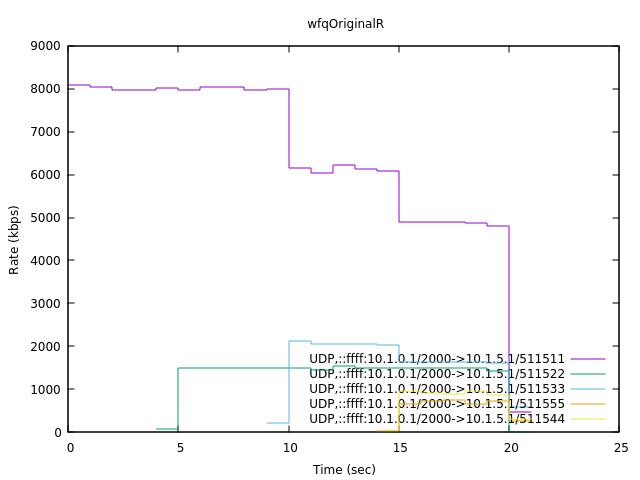
\includegraphics[width=0.6\linewidth]{wfqOriginalR.png}
                \caption{Tasa de cada flujo.}
                \label{fig:wfqOriginalR}
            \end{figure}

            \begin{figure}
                \centering
                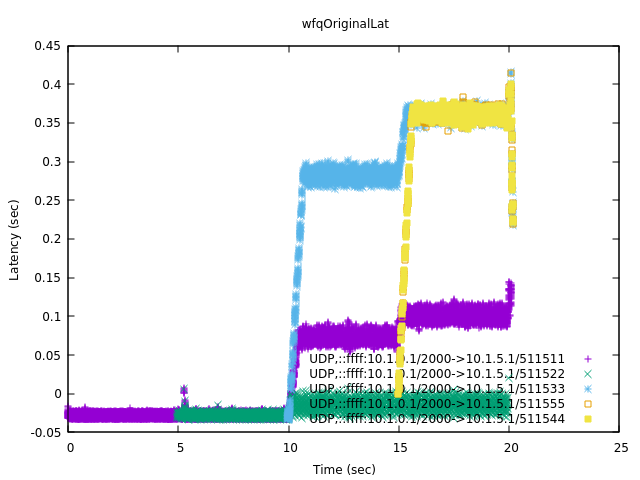
\includegraphics[width=0.6\linewidth]{wfqOriginalLat.png}
                \caption{Latencia de cada flujo.}
                \label{fig:wfqOriginalLat}
            \end{figure}

    \section{Garantizando una latencia mínima con \textit{WFQ} (2.1.2)}
        Empleando los mismos flujos que en el apartado anterior vamos a priorizar uno de los flujos de manera que solo se saquen paquetes de otras colas si y solo si esta cola prioritaria está vacía. Como esto podría provocar inanición, la implementación práctica descartará el tráfico prioritario en exceso (según el porcentaje configurado) a no ser que las demás colas estén vacías. Ésto se traducirá en que se mantendrá una latencia acotada pero se incrementarán las pérdidas del flujo prioritario a medida que se añadan más flujos a la prueba. La configuración del router para este caso se puede encontrar \href{https://github.com/UAH-s-Telematics-Engineering-Tasks/traff_eng/blob/master/P2/Router_confs/prioWFQ.cfg}{aquí}, siendo la única diferencia con la anterior la línea \texttt{58}.

        \subsection{Comentando las figuras}
            Tal y como comentábamos al explicar la implementación de las prioridades observamos cómo la tasa del flujo prioritario (el \texttt{1}) empezará en los $8\ Mbps$ iniciales hasta que se incorporan más flujos. Al hacerlo, la tasa se irá reduciendo hasta que en los últimos $5\ segundos$ se aproxima a $1\ Mbps$, el $10\%$ de la velocidad del interfaz que configuramos. Todo esto se observa en la figura \ref{fig:wfqPrioR}.\\

            Si observamos la latencia en la figura \ref{fig:wfqPrioLat} nos daremos cuenta de que, como antes, la latencia del flujo \texttt{2} se mantiene constante al tener asignado suficiente ancho de banda y que \textbf{además} la latencia del flujo \texttt{1} también está acotada al ser el flujo prioritario. Las demás tasas se comportan como comentábamos antes.\\

            Si acabamos por observar las pérdidas en la figura \ref{fig:wfqPrioLoss} nos daremos cuenta de que las pérdidas de todos los flujos excepto el \texttt{2} experimentarán pérdidas hacia el final de la prueba. Si nos centramos en el flujo \texttt{1}, el prioritario, veremos que estas pérdidas comienzan a dispararse en cuanto el tercer flujo entra en acción y debemos empezar a descartar paquetes. Es interesante ver que el aumento de las pérdidas del flujo \texttt{1} se produce en el mismo instante en el que su tasa se disminuye.

            \begin{figure}
                \centering
                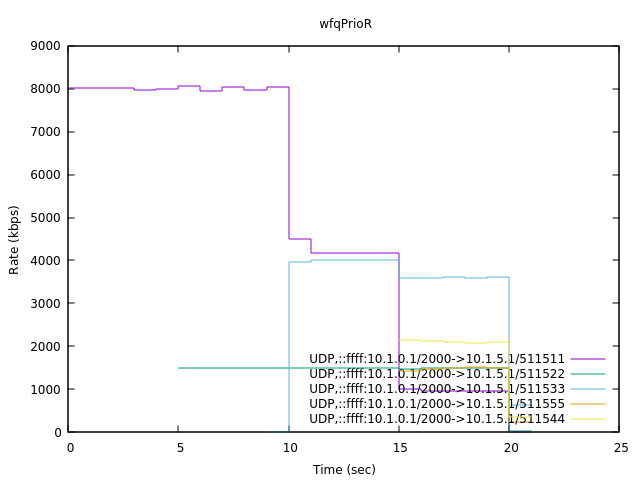
\includegraphics[width=0.6\linewidth]{wfqPrioR.png}
                \caption{Tasa de cada flujo.}
                \label{fig:wfqPrioR}
            \end{figure}

            \begin{figure}
                \centering
                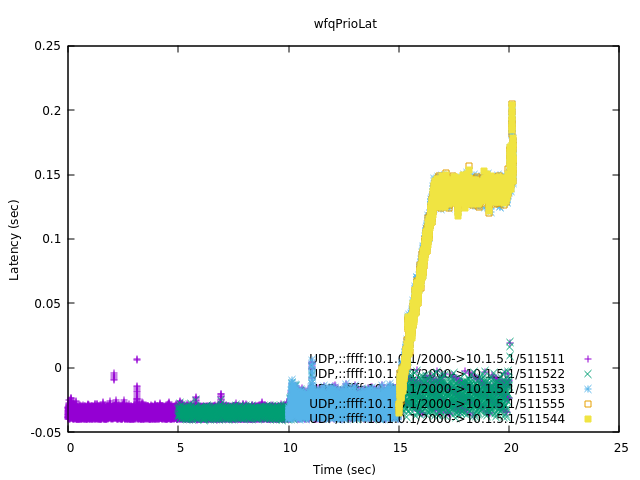
\includegraphics[width=0.6\linewidth]{wfqPrioLat.png}
                \caption{Latencia de cada flujo.}
                \label{fig:wfqPrioLat}
            \end{figure}

            \begin{figure}
                \centering
                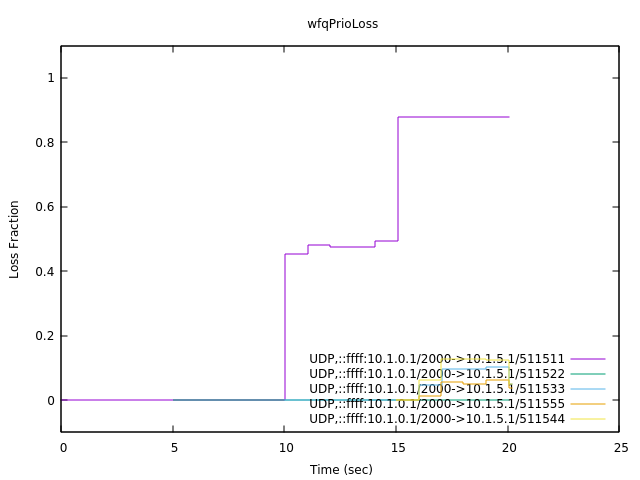
\includegraphics[width=0.6\linewidth]{wfqPrioLoss.png}
                \caption{Pérdidas de cada flujo.}
                \label{fig:wfqPrioLoss}
            \end{figure}

    \section{Garantizando una latencia mínima con \textit{WFQ} y vigilancia (2.1.3)}
        Empleando los mismos flujos que en los apartados anteriores vamos a añadir una ``capa'' de \textit{vigilancia} que se encargará de que el tráfico sobrante del flujo prioritario sea descartado sin importar si las demás colas están vacías o no. Ésto nos podría evitar problemas con el tráfico extra ya que éste entraría en colas que estuvieran vacías en ese momento... Para lograrlo configuraremos una función \textit{policía} en la \textit{clase} asociada al flujo \texttt{1}. Que rechazará el tráfico sobrante por encima de la tasa asignada a dicha \textit{clase}. Como hemos asignado al flujo prioritario un $10\%$ de la capacidad de la interfaz ($V_l = 10\ Mbps$) éste contará con una tasa de $1\ Mbps$. Ésta tasa será la que utilizaremos como límite en la función \textit{policía} que hemos de configurar. Dicha configuración se puede encontrar en la línea \texttt{64} de \href{https://github.com/UAH-s-Telematics-Engineering-Tasks/traff_eng/blob/master/P2/Router_confs/policeWFQ.cfg}{éste} archivo.

        \subsection{Comentando las figuras}
            Observando la figura \ref{fig:wfqPoliceR} nos damos cuenta de que, a diferencia del caso anterior, la tasa del flujo prioritario se limita prácticamente desde el inicio de la prueba. Al no haber especificado el valor de \texttt{BE}, la cantidad de datos que pueden rebasar la \texttt{CIR} momentáneamente (el tamaño de un cubo de créditos asociado a la función de \textit{policiía}), creemos que un valor por defecto distinto de $0$ puede ser la causa del pico inicial superior a $1\ Mbps$. En cualquier caso, podemos considerar que la tasa está limitada a $1\ Mbps$ durante la duración de la prueba, cosa que diferencia este caso y el anterior totalmente.\\

            Si ahora estudiamos la figura \ref{fig:wfqPoliceLat} veremos que es prácticamente idéntica a la del caso anterior. La única diferencia con el escenario sin función de \textit{policía} es que limitamos la tasa del flujo prioritario desde el principio. No obstante, como el flujo prioritario era ``desalojado'' por los demás hasta que la tasa asociada era la mínima garantizada (el $10\%$) no observamos diferencias en la latencia en ningún caso.\\

            Finalmente podemos analizar las pérdidas de cada flujo en la figura \ref{fig:wfqPoliceLoss}. La diferencia con el caso anterior es que la pérdida de paquetes del flujo prioritario es muy elevada desde el primer instante además de ser constante. La ``simetría'' con la tasa del mismo flujo se aprecia de nuevo al igual que en el caso anterior: como empezamos a descartar tráfico desde prácticamente el principio la tasa es elevada desde ese mismo instante. La relación que existía en el caso anterior se mantiene pero es diferente a este caso porque la evolución de la tasa del flujo prioritario es también diferente al haber aplicado al función \textit{policía}.

            \begin{figure}
                \centering
                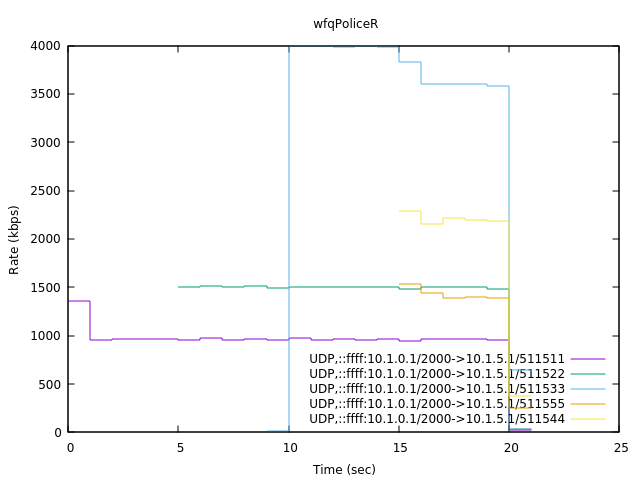
\includegraphics[width=0.6\linewidth]{wfqPoliceR.png}
                \caption{Tasa de cada flujo.}
                \label{fig:wfqPoliceR}
            \end{figure}

            \begin{figure}
                \centering
                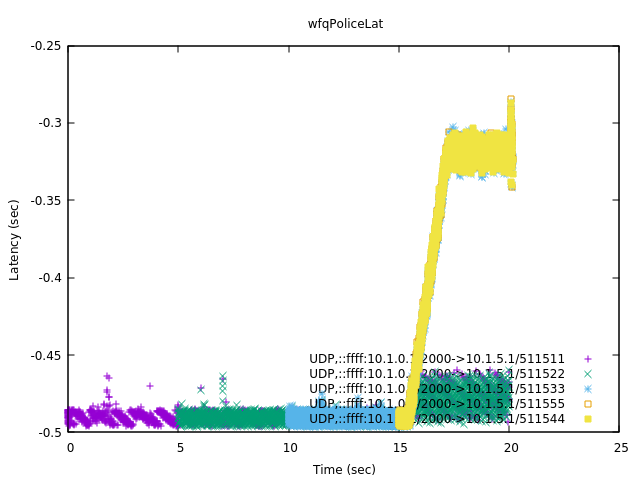
\includegraphics[width=0.6\linewidth]{wfqPoliceLat.png}
                \caption{Latencia de cada flujo.}
                \label{fig:wfqPoliceLat}
            \end{figure}

            \begin{figure}
                \centering
                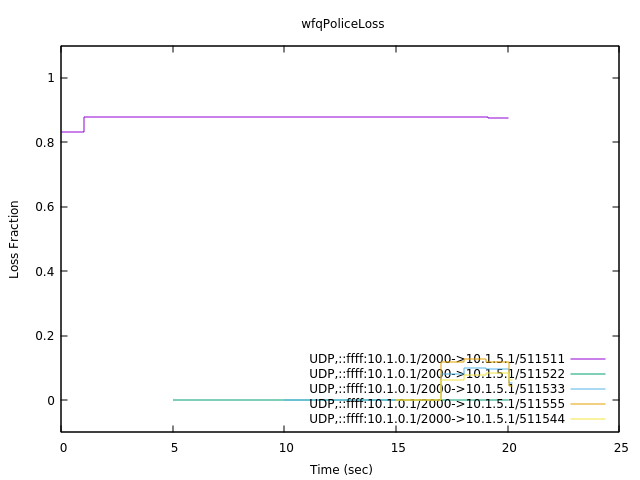
\includegraphics[width=0.6\linewidth]{wfqPoliceLoss.png}
                \caption{Pérdidas de cada flujo.}
                \label{fig:wfqPoliceLoss}
            \end{figure}

    \section{Cálculos teóricos sobre un planificador}
        En esta sección resolvemos el ejercicio con resultados propuesto en el guión. En nuestro caso contamos con un enlace de velocidad $V_l = 10\ Mbps$ y $5\ flujos$ de $2,\ 1,\ 2,\ 3\ y\ 4\ Mbps$ cuya capacidad asignada es $15\%,\ 40\%,\ 10\%,\ 10\%\ y\ 25\%$, respectivamente. Incluimos las tablas \ref{tab:iter1}-\ref{tab:iter3} así como los grupos de ecuaciones \ref{eq:iter1}-\ref{eq:iter3} con cada una de las iteraciones. Los resultados aparecen en la tabla \ref{tab:results}.

        \begin{table}
            \centering
            \begin{tabular}{|c|c|c|c|c|}
                \hline
                \texttt{Peso (\%)} & \texttt{Tráfico Inicial [Mbps]} & \texttt{C. min. g. [Mbps]} & \texttt{C. Asig. [Mbps]} & \texttt{T. Pend. [Mbps]}\\
                \hline
                15 & 2 & 1,5 & 1,5 & 0,5\\
                \hline
                40 & 1 & 4 & 1 & 0\\
                \hline
                10 & 2 & 1 & 1 & 1\\
                \hline
                10 & 3 & 1 & 1 & 2\\
                \hline
                25 & 4 & 2,5 & 2,5 & 1,5\\
                \hline
            \end{tabular}
            \caption{Primera iteración.}
            \label{tab:iter1}
        \end{table}

        \begin{align} \label{eq:iter1}
            C_{min_i} &= V_l \cdot \frac{w_i}{\sum_{i = 1}^5 w_i}\\
            C_{min_1} &= 10\ Mbps \cdot \frac{15}{100} = 1,5\ Mbps\\
            C_{min_2} &= 10\ Mbps \cdot \frac{40}{100} = 4\ Mbps\\
            C_{min_3} &= 10\ Mbps \cdot \frac{10}{100} = 1\ Mbps\\
            C_{min_4} &= 10\ Mbps \cdot \frac{10}{100} = 1\ Mbps\\
            C_{min_5} &= 10\ Mbps \cdot \frac{25}{100} = 2,5\ Mbps
        \end{align}

        \begin{table}
            \centering
            \begin{tabular}{|c|c|c|c|c|}
                \hline
                \texttt{Peso (\%)} & \texttt{T. Pend. I. [Mbps]} & \texttt{C. min. g. [Mbps]} & \texttt{C. Asig. [Mbps]} & \texttt{T. Pend. F. [Mbps]}\\
                \hline
                15 & 0,5 & 0,75 & 0,5 & 0\\
                \hline
                & 0 & & 0 & 0\\
                \hline
                10 & 1 & 0,5 & 0,5 & 0,5\\
                \hline
                10 & 2 & 0,5 & 0,5 & 1,5\\
                \hline
                25 & 1,5 & 1,25 & 1,25 & 0,25\\
                \hline
            \end{tabular}
            \caption{Segunda iteración.}
            \label{tab:iter2}
        \end{table}

        \begin{align} \label{eq:iter2}
            C_{sobrante} &=  10 - (1,5 + 1 + 1 + 1 + 2,5) = 3\ Mbps\\
            C_{min_1} &= 3\ Mbps \cdot \frac{15}{60} = 0,75\ Mbps\\
            C_{min_3} &= 3\ Mbps \cdot \frac{10}{60} = 0,5\ Mbps\\
            C_{min_4} &= 3\ Mbps \cdot \frac{10}{60} = 0,5\ Mbps\\
            C_{min_5} &= 3\ Mbps \cdot \frac{25}{60} = 1,25\ Mbps
        \end{align}

        \begin{table}
            \centering
            \begin{tabular}{|c|c|c|c|c|}
                \hline
                \texttt{Peso (\%)} & \texttt{T. Pend. I. [Mbps]} & \texttt{C. min. g. [Mbps]} & \texttt{C. Asig. [Mbps]} & \texttt{T. Pend. F. [Mbps]}\\
                \hline
                & 0 & & 0 & 0\\
                \hline
                & 0 & & 0 & 0\\
                \hline
                10 & 0,5 & 0,056 & 0,056 & 0,444\\
                \hline
                10 & 1,5 & 0,056 & 0,056 & 1,444\\
                \hline
                25 & 0,25 & 0,139 & 0,139 & 0,111\\
                \hline
            \end{tabular}
            \caption{Tercera iteración.}
            \label{tab:iter3}
        \end{table}

        \begin{align} \label{eq:iter3}
            C_{sobrante} &=  3 - (0,5 + 0,5 + 0,5 + 1,25) = 0,25\ Mbps\\
            C_{min_3} &= 0,25\ Mbps \cdot \frac{10}{45} = 0,056\ Mbps\\
            C_{min_4} &= 0,25\ Mbps \cdot \frac{10}{45} = 0,056\ Mbps\\
            C_{min_5} &= 0,25\ Mbps \cdot \frac{25}{45} = 0,139\ Mbps
        \end{align}

        Con la tercera iteración recogida en la tabla \ref{tab:iter3} terminamos el reparto ya que ninguno de los flujos restantes recibe tanta capacidad como tráfico pendiente. Por lo tanto, el reparto queda:

        \begin{table}
            \centering
            \begin{tabular}{|c|c|}
                \hline
                \texttt{Flujo} & \texttt{Capacidad asignada [Mbps]}\\
                \hline
                1 & $1,5 + 0,5 = 2$\\
                \hline
                2 & $1$\\
                \hline
                3 & $1 + 0,5 + 0,056 = 1,556$\\
                \hline
                4 & $1 + 0,5 + 0,056 = 1,556$\\
                \hline
                5 & $2,5 + 1,25 + 0,139 = 3,889$\\
                \hline
            \end{tabular}
            \caption{Resultados tras el reparto.}
            \label{tab:results}
        \end{table}

    \section{Cubos con créditos (2.3)}
        En esta sección estudiamos el conformado de tráfico con un \textit{cubo de créditos} para después aplicar una función \textit{policía}.

        \subsection{Prueba de conformado (2.3.1)}
            Incluimos la entrada de la ráfaga descrita en esta sección y la siguiente, así como la salida esperada para el \textit{cubo de créditos} en las figuras \ref{fig:inputBucks} y \ref{fig:outputBucks}, respectivamente.\\

            \begin{figure}
                \centering
                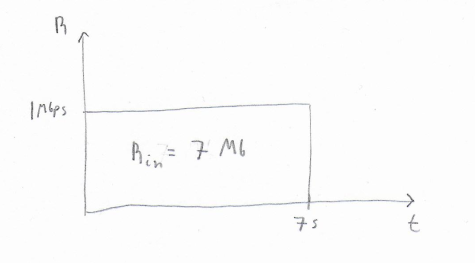
\includegraphics[width=0.6\linewidth]{tokenBucketsInput.png}
                \caption{Entrada de ambos sistemas.}
                \label{fig:inputBucks}
            \end{figure}

            \begin{figure}
                \centering
                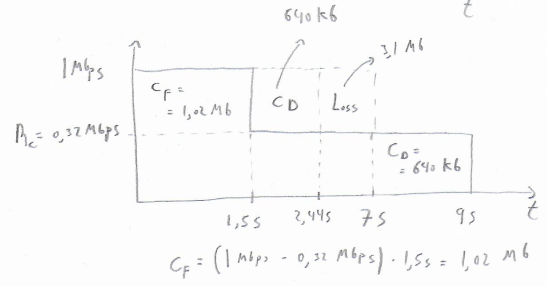
\includegraphics[width=0.6\linewidth]{tokenBucketsOutput.png}
                \caption{Salida esperada del \textit{cubo de créditos}.}
                \label{fig:outputBucks}
            \end{figure}

            La configuración del encaminador se incluye en \href{https://github.com/UAH-s-Telematics-Engineering-Tasks/traff_eng/blob/master/P2/Router_confs/tokenBucket.cfg}{éste} archivo. Como la prueba solo contiene un flujo empleamos la clase por defecto del encaminador para facilitar la sintaxis de configuración.\\

            Incluimos la tasa de salida de la ráfaga conformada en la figura \ref{fig:tokenBucketR}. Esperamos que la tasa caiga hasta la velocidad media en $t = 1,5\ s$ pero dado que la granularidad de \texttt{trpr} es de $1\ s$ veremos la caída en $t = 1\ s$


\end{document}
